\documentclass{beamer} 
\usetheme{metropolis}
% \usecolortheme{spruce}
\setlength{\parindent}{0cm}
\usepackage{color}
\usepackage[utf8]{inputenc}
\usepackage[spanish]{babel}
\usepackage{amsmath}
\usepackage{amsfonts}
\usepackage{amssymb}
\usepackage{graphicx}
\usepackage{ragged2e}
\usepackage{caption}
\usepackage{subcaption}
\usepackage{tikz}
\usepackage{tcolorbox}
\usepackage{float}

\newtcolorbox{informacion}[2][]
{
  breakable,
  colframe = blue!5!white,
  colback  = blue!5!white,
  coltitle = blue!80!black,
  title    = \faInfo \hspace{5 mm} #2,
}


\title{Torsión}
\author{Pedro Jorge De Los Santos}
\institute{
    {\bf 
    Instituto Tecnológico de Celaya \\
    Departamento de Ingeniería Mecánica \\
    }
}

\apptocmd{\frame}{}{\justifying}{}
\begin{document}

\begin{frame}
\titlepage
\end{frame}

% Sección introducción
\section{Introducción}

\begin{frame}
\justifying
\frametitle{Torsión}

\begin{center}
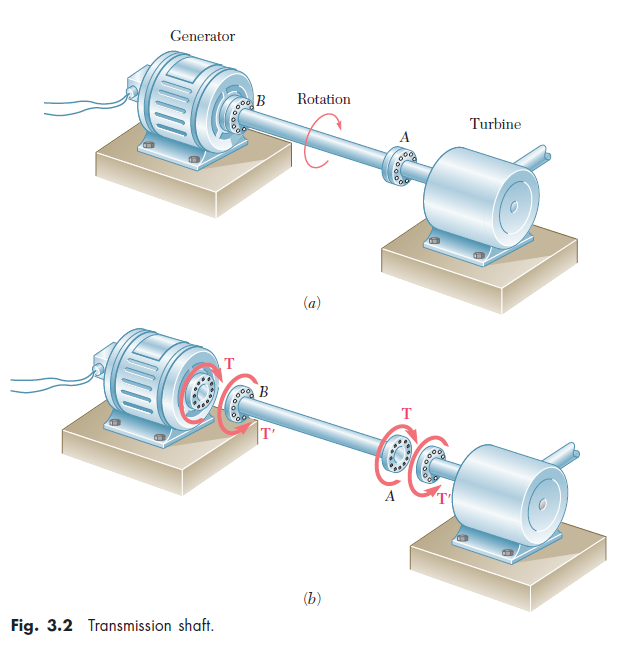
\includegraphics[width=0.6\textwidth]{img/flecha_transmision.PNG}
\end{center}

\end{frame}


\begin{frame}
\justifying
\frametitle{Análisis preliminar de esfuerzos}

Consideremos un eje sometido a torsión. Efectuando un corte perpendicular:

\begin{center}
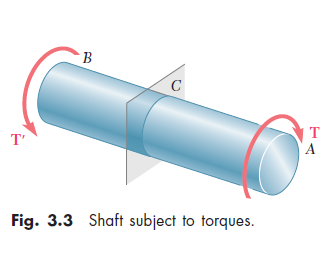
\includegraphics[width=0.55\textwidth]{img/shaft_torque.PNG}
\end{center}

\end{frame}


\begin{frame}
\justifying
\frametitle{Análisis preliminar de esfuerzos}

\begin{center}
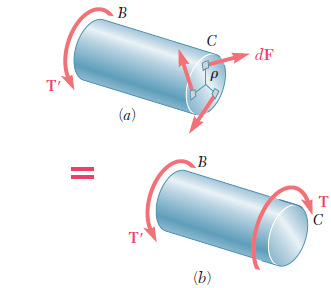
\includegraphics[width=0.35\textwidth]{img/shaft_torque_diagram.PNG}
\end{center}

$$ \int \rho \, dF = T $$

dado que $dF = \tau \, dA$, entonces:

$$ \int \rho \, (\tau \, dA) = T $$

\end{frame}


\begin{frame}
\justifying
\frametitle{Deformaciones en un eje circular}

\begin{center}
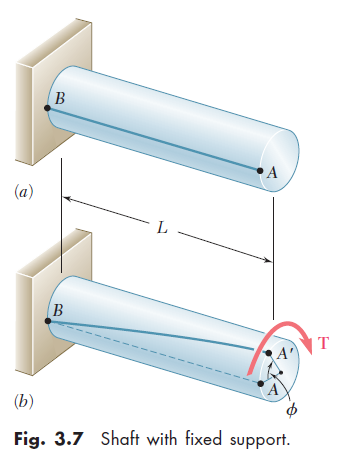
\includegraphics[width=0.35\textwidth]{img/shaft_fixed.PNG}
\end{center}

\begin{itemize}
\item $\phi$  - Ángulo de giro
\item $L$ - Longitud
\item $T$ - Par de torsión
\end{itemize}

% Necesitamos determinar una relación entre las tres variables anteriores.

\end{frame}


\begin{frame}
\justifying
\frametitle{Deformaciones en un eje circular}

\begin{center}
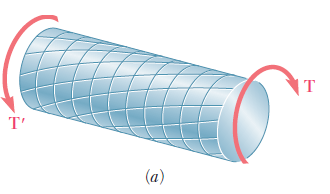
\includegraphics[width=0.45\textwidth]{img/shaft_deformations.PNG}
\end{center}

\begin{informacion}{Propiedades de ejes sometidos a torsión}
Cuando un eje circular se somete a torsión todas sus secciones transversales permanecen planas y 
sin distorsión.
\end{informacion}

\end{frame}


\begin{frame}
\justifying
\frametitle{Deformaciones en un eje circular}


\begin{minipage}{\linewidth}
  \centering
  \begin{minipage}{0.45\textwidth}
  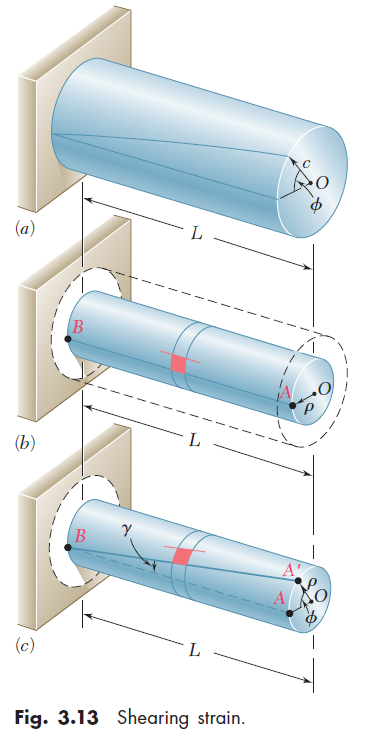
\includegraphics[width=0.85\textwidth]{img/shearing_strain.PNG}
  \end{minipage}
  \hspace{0.05\linewidth}
  \begin{minipage}{0.45\linewidth}
  Para valores pequeños de $\gamma$, puede expresarse la longitud de arco AA' como $AA' = L\gamma $, pero también 
  se tiene que $AA' = \rho \phi$, entonces, $L\gamma = \rho\phi$, o:

  $$ \gamma =\frac{\rho\phi}{L} $$
  \end{minipage}
\end{minipage}

\end{frame}


\begin{frame}
\justifying
\frametitle{Deformaciones en un eje circular}

La deformación a cortante es máxima en la superficie del eje, en donde $\rho = c$, entonces:

$$ \gamma_{max} = \frac{c\phi}{L} $$

Aplicando un poco de álgebra se tiene:

$$ \gamma = \frac{\rho}{c} \gamma_{max} $$

\end{frame}


\begin{frame}
\justifying
\frametitle{Esfuerzos en el rango elástico}

Ley de Hooke para esfuerzos a cortante:

$$\tau = G \gamma $$

Multiplicando la ecuación obtenida para $\gamma$ por G, se tiene:

$$ G\gamma = \frac{\rho}{c} G \gamma_{max} $$

$$ \tau = \frac{\rho}{c} \tau_{max} $$

\end{frame}


\begin{frame}
\justifying
\frametitle{Esfuerzos en el rango elástico}

\begin{center}
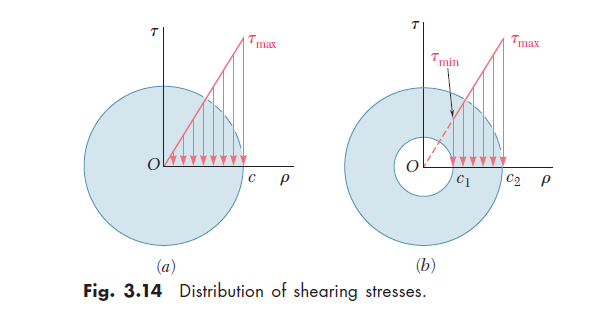
\includegraphics[width=0.75\textwidth]{img/stress_distribution.PNG}
\end{center}

$$ \tau_{min} = \frac{c_1}{c_2} \tau_{max} $$

\end{frame}


\begin{frame}
\justifying
\frametitle{Esfuerzos en el rango elástico}

De la formulación infinitésimal se tiene:

$$ T = \int \rho \tau \, dA = \frac{\tau_{max}}{c} \int \rho^2 \, dA $$

donde $\int \rho \, dA = J$, siendo $J$ el momento polar de inercia respecto a $O$. Así:

$$ T = \frac{\tau_{max} J}{c}  \,\,\,\, \rightarrow \,\,\,\, \tau_{max} = \frac{Tc}{J} $$

Generalizando:

$$ \tau = \frac{T\rho}{J} $$

\end{frame}









\end{document}

